\documentclass[10pt,a4paper]{article}
\usepackage[margin=15mm,top=14mm,bottom=12mm]{geometry}
\usepackage{graphicx,amsmath,booktabs,enumitem,xcolor}
\usepackage[colorlinks=true,linkcolor=black,urlcolor=black]{hyperref}
\pagestyle{empty}
\setlength{\parindent}{0pt}\setlength{\parskip}{2pt}
\setlist{itemsep=0.5pt,topsep=1pt,leftmargin=12pt}
\definecolor{mid}{HTML}{6E6E6E}
\begin{document}
{\large\bfseries One constant per hydroxyl group: predicting freeze concentration and designing glycerol-sparing cryoprotectants}\\[1pt]
{\small Siddhant Chowdhary, 25B0347 \quad$\cdot$\quad CL207 optional project \quad$\cdot$\quad \textbf{Checkpoint 3 summary} (full draft: 5-page document)}
\vspace{2pt}\hrule\vspace{4pt}

\begin{minipage}[t]{0.56\textwidth}
\textbf{Question.} When cells freeze, ice is pure water, so salt concentrates in the liquid left behind. Ice--solution
equilibrium fixes the water activity of that liquid at each temperature,
$\ln(x_w\gamma_w) = -\tfrac{\Delta_{\rm fus}H}{R}\big(\tfrac1T-\tfrac1{T_m}\big) - \Delta C_p\text{ term}$,
so the only unknown is $\gamma_w$. How little glycerol keeps the salt below the damage level, and how much of it can sorbitol replace?

\textbf{Hypothesis (tested, not assumed).} One water--OH interaction constant, $\ln\gamma_w = (1-x_w)\sum_i \frac{n_{{\rm OH},i}\,a_{\rm OH}}{RT}x_i$,
fitted on glycerol only, predicts other polyols and polyol\,+\,salt mixtures without refitting.

\textbf{How.} Fit $a_{\rm OH} = -2415$\,J\,mol$^{-1}$ on 19 CRC glycerol points (RMSE 0.017\,K) $\rightarrow$ predictions
committed to git $\rightarrow$ compared with independent literature data and five benchmark models $\rightarrow$ recipe.
Everything rebuilds from one command (\texttt{run\_all.py}).
\end{minipage}\hfill
\begin{minipage}[t]{0.42\textwidth}
\vspace{-6pt}
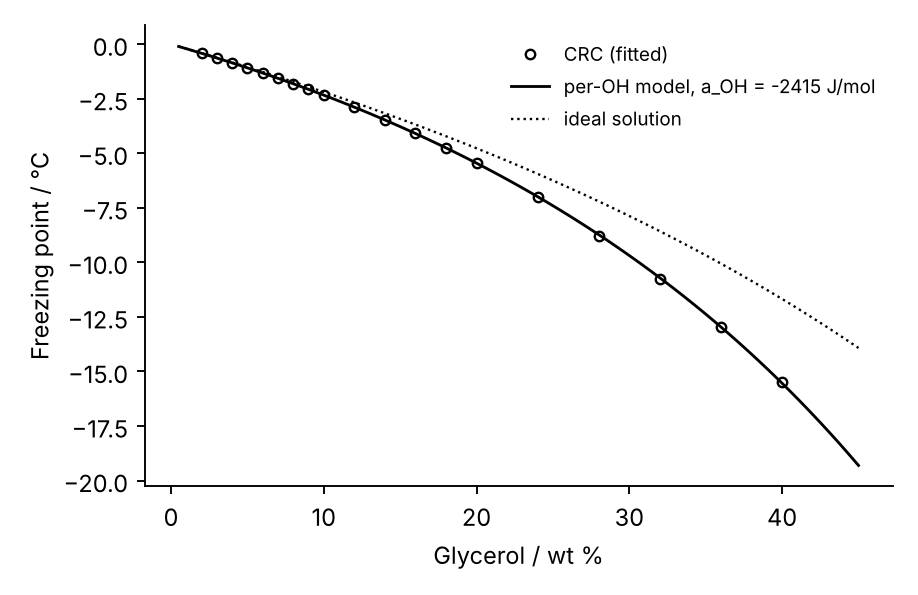
\includegraphics[width=\textwidth]{fit_glycerol.png}\\[-2pt]
{\footnotesize\textbf{Fig.\ 1.} The only fit: glycerol, one constant.}
\end{minipage}

\vspace{3pt}
\includegraphics[width=\textwidth]{report_results.png}\\[-1pt]
{\footnotesize\textbf{Fig.\ 2.} (a) Blind single-solute tests (log scale). (b) Glycerol\,+\,NaCl liquidus (Shepard 1976): our additive rule vs the two
cryobiology models. (c) Glycerol needed vs sorbitol added, three activity models, $-15$\,\textdegree C, NaCl $\le$ 4.41\,wt\%.}

\vspace{3pt}
\begin{minipage}[t]{0.52\textwidth}
\textbf{Results so far}
\begin{itemize}
\item \textbf{Transfers:} ethylene glycol 0.83\,K (ideal 2.49, UNIFAC 3.99); sucrose 0.02\,K (ideal 0.35).
\item \textbf{Mixtures:} glycerol\,+\,NaCl above 30\,wt\% solute 1.23\,K vs osmotic virial 5.75 and Kleinhans--Mazur 3.39.
Below 30\,wt\%: 0.69\,K, a narrow miss of our pre-set 0.5\,K target.
\item \textbf{Fails:} sorbitol (concentrated, and at 25\,\textdegree C) and monohydric alcohols. A sucrose two-temperature test shows the
sorbitol failure is the molecule, not temperature.
\item \textbf{UNIFAC} predicts the wrong sign of non-ideality for water--glycerol.
\item \textbf{Design:} 1\,g sorbitol saves 0.68--0.91\,g glycerol across 3 models $\times$ 3 temperatures $\times$ 3 salt limits.
\item \textbf{Effort note:} Shepard (1976) gives no tables; its Fig.\ 3 was digitised by hand (76 points, checked against the
NaCl--water eutectic; figure accuracy measured at 0.34\,K against CRC).
\end{itemize}
\end{minipage}\hfill
\begin{minipage}[t]{0.45\textwidth}
\textbf{Next (before 6 Nov)}
\begin{itemize}
\item Lab: 5 committed samples in duplicate; expected $U \approx 0.25$\,K vs model spreads 0.7--6.6\,K.
\item UNIFAC cross-check in DWSIM; post-hoc per-molecule fit, labelled as such.
\end{itemize}
\textbf{Feedback I would like}
\begin{enumerate}
\item Is reporting the failures (sorbitol, alcohols, the 0.5\,K miss) as results the right framing for this proposal?
\item Lab: dates; is a conductivity meter or refractometer available to measure salt in the unfrozen liquid?
\item Is a post-hoc section fine in the 5 pages, or should it be an appendix?
\item May the 5 pages use a journal-paper layout, keeping your section order?
\item Aspen Plus access for the UNIFAC check?
\end{enumerate}
\end{minipage}
\end{document}
